\documentclass[12pt]{article}
\usepackage{amsmath}
\usepackage{amsfonts}
\usepackage{float}
\usepackage{tikz}
\usepackage{graphicx}
\usepackage{enumerate}
\usepackage{mathrsfs}

\usepackage{adjustbox}
\usetikzlibrary{arrows.meta, automata, positioning,decorations.pathreplacing, decorations.markings}
\usepackage{pgfplots}
\pgfplotsset{compat=1.17}
\usepackage{enumitem} % For custom list formatting
\usepackage{tikz}
\usepackage{amsmath}
\usetikzlibrary{calc}

\title{MATH381 Assignment 3}
\author{Ben Vickers}
\date{Due: 11:55 PM, Thursday 19 September 2024}

\begin{document}

\maketitle

\noindent \textbf{Q1.} Evaluate \(\int_{\gamma} z \overline{z} \, dz\) where \(\gamma\) is a closed curve that traverses the boundary of the half annulus \(\{ z : 1 < |z| < 2 \text{ and } \operatorname{Im}(z) > 0 \}\) once in an anti-clockwise direction.

\noindent \textit{Hint: The integrand is not holomorphic, so most integral theorems don’t apply and you’ll need to use the definition of an integral over a curve.}
\[\]

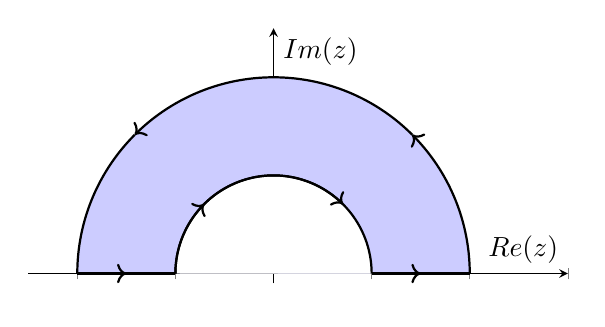
\begin{tikzpicture}
    \begin{axis}[
        axis equal image,
        xmin=-2.5, xmax=3,
        ymin=-0.1, ymax=2.5,
        xlabel=$Re(z)$,
        xlabel style={xshift=6}, % Move xlabel further right
        ylabel=$Im(z)$,
        axis lines=middle,
        samples=200,
        domain=-2:2,
        yticklabels={},
        xticklabels={}
    ]
    % Plot the outer boundary (|z| = 2) with filling
    \addplot[domain=0:180, samples=100, fill=blue!20, draw=none] 
        ({2*cos(x)}, {2*sin(x)});

    % Plot the inner boundary (|z| = 1) with filling
    \addplot[domain=0:180, samples=100, fill=white, draw=none] 
        ({cos(x)}, {sin(x)});

    % Draw the outer boundary (|z| = 2) with arrows
    \addplot[domain=0:45, thick, ->] 
        ({2*cos(x)}, {2*sin(x)});
    \addplot[domain=45:135, thick, ->] 
        ({2*cos(x)}, {2*sin(x)});
    \addplot[domain=135:180, thick] 
        ({2*cos(x)}, {2*sin(x)});

    % Draw the inner boundary (|z| = 1) with arrows
    \addplot[domain=180:135, thick, ->] 
        ({cos(x)}, {sin(x)});
    \addplot[domain=135:45, thick, ->] 
        ({cos(x)}, {sin(x)});
    \addplot[domain=0:180, thick] 
        ({cos(x)}, {sin(x)});

    % Draw the highlighted parts of the x-axis
    \draw[thick, black] (-2,0) -- (-1,0);
    \draw[thick, black] (1,0) -- (2,0);

    % Draw arrow in the middle of the line from -2 to -1
    \draw[thick, black, ->] (-2,0) -- (-1.5,0);

    % Draw arrow in the middle of the line from -2 to -1
    \draw[thick, black, ->] (1,0) -- (1.5,0);

    \end{axis}
\end{tikzpicture}
\newline
\linebreak
\noindent We take \(\gamma\) to be the joining of \(\gamma_1, \gamma_2, \gamma_3, \gamma_4\) defined as follows:
\begin{enumerate}
\item \(\gamma_1 = t, \, t \in \left[1,2\right]\) 
\item \(\gamma_2 = 2e^{it}, \, t \in \left[0, \pi\right]\) 
\item \(\gamma_3 = t, \, t \in \left[-2,-1\right]\) 
\item \(\gamma_4 = e^{it}, \, t \in \left[\pi, 0\right]\) 
\end{enumerate}
\vspace{0.1cm}
\noindent Now by \(\textbf{Proposition 7.20}\) we can take the integral over \(\gamma\) to be the sum of the integrals over the four component curves of \(\gamma\) as \(f(z) = z \overline{z} = \left|z\right|^2\) is continuous on \(\mathbb{C}\) and more specifically on \(\gamma\). \newline
\linebreak
\noindent Namely we can apply the following:
\begin{enumerate}
    \item \(\int_{\gamma} f(z) \, dz := \int_{a}^{b} f(\gamma(t)) \, \gamma'(t) \, dt \,\)
    \item \(\int_{\gamma} f(z) \, dz = \int_{\gamma_1} f(z) \, dz + \cdots + \int_{\gamma_4} f(z) \, dz\)
\end{enumerate}


\noindent Which obtains the following result:
\[
\int_{\gamma_1} f(z) \, dz = \int_{1}^{2} f(t) \cdot 1 \, dt =  \int_{1}^{2} t \cdot t \, dt =  \int_{1}^{2} t^2 \, dt = \frac{7}{3}
\]
\[
\int_{\gamma_2} f(z) \, dz = \int_{0}^{\pi} f(2e^{it})\cdot 2ie^{it} \, dt = \int_{0}^{\pi} 2e^{-it} \cdot 2e^{it }\cdot 2ie^{it} \, dt = 8i \int_{0}^{\pi} e^{it}
\]
\[
= 8i \cdot \frac{1}{i} \left[e^{it}\right]_{0}^{\pi} = 8 \cdot \left[-1 - 1\right] = 8 \cdot \left[-2\right] = -16
\]
\[
\int_{\gamma_3} f(z) \, dz = \int_{-2}^{-1} f(t) \, dt =  \int_{-2}^{-1} t \cdot t \, dt =  \int_{-2}^{-1} t^2 \, dt = \frac{7}{3}
\]
\[
\int_{\gamma_4} f(z) \, dz = \int_{\pi}^{0} f(e^{it})\cdot ie^{it} \, dt = \int_{\pi}^{0}e^{-it} \cdot e^{it}\cdot ie^{it} \, dt = i \int_{\pi}^{0} e^{it} = -i \int_{0}^{\pi} e^{it} = -i \cdot 2i = 2
\]
\[
\implies \int_{\gamma} f(z) \, dz = \frac{7}{3} -16 + \frac{7}{3} + 2 + \frac{7}{3} = \frac{14}{3} -14 = \frac{-28}{3}
\]
\[\]
\textbf{Q2.} Evaluate the following integrals:
\begin{itemize}
    \item[(i)] \(\int_{\gamma} 2z^3 - 5z^2 + z + 4 \, dz\) where \(\gamma = \overline{[2, 3i]}\).
    \item[(ii)] \(\int_{\gamma} (z - 3)^8 \, dz\) where \(\gamma\) is the clockwise circular arc from \(3 + 2i\) to \(3 - 2i\) having radius \(\sqrt{13}\) centred at the origin.
    \item[(iii)] \(\int_{\gamma} \cos(z) e^{i\pi \sin(z)} \, dz\) where \(\gamma(t) = \frac{\pi}{2} t + it(1 - t)\) for \(t \in [0, 1]\).
\end{itemize}

\noindent \textit{Hint: Use the Fundamental Theorem of Calculus for curves where possible.}\newline
\noindent \begin{enumerate}[label=\textbf{(\roman*)}]
 \item By the FTC (\(\textbf{Theorem 8.3}\)) we have that as \(f\) is continuous on \(\mathbb{C} \supset \gamma\) (by the continuity of polynomials), and there exists \(F\) such that \(F' = f\) then \(\int_{\gamma} f(z) \, dz = F(\gamma(b)) - F(\gamma(a))\) 

 We have:
 \[F(z) = \int_{0}^{z} 2s^3 - 5s^2 + s + 4 \, ds = \frac{1}{2}z^4 -\frac{5}{3}z^3 + \frac{1}{2}z^2 + 4z\]
 \[\implies \int_{\gamma} 2z^3 - 5z^2 + z + 4 \, dz = \left[  \frac{1}{2}z^4 -\frac{5}{3}z^3 + \frac{1}{2}z^2 + 4z\right]_{2}^{3i} \]
 \[= \left[\frac{81}{2} +\frac{135i}{3} -\frac{9}{2} +12i\right] - \left[8-\frac{40}{3}+2+8\right]\]
 \[= \frac{94}{3} + \frac{171i}{3} \]
 \[= \frac{94}{3} \,+ \,57i \]

 \item We can notice that as \(f\) is a polynomial in \(z\), it is holomorphic in \(\mathbb{C}\) and for the sake of the next step, holomorphic in say the open disk, \(D(0,999) \subset \mathbb{C}\). 

 We can now apply \(\textbf{Corollary 8.2}\) which states that if \(f\) is holomorphic in an open disk \(D\) and there exists two curves, \(\gamma \text{ and } \sigma\) in \(D\) with the same start and end points then:
 \[
 \int_{\gamma} f(z)\,dz = \int_{\sigma} f(z) \, dz.
 \]

 

 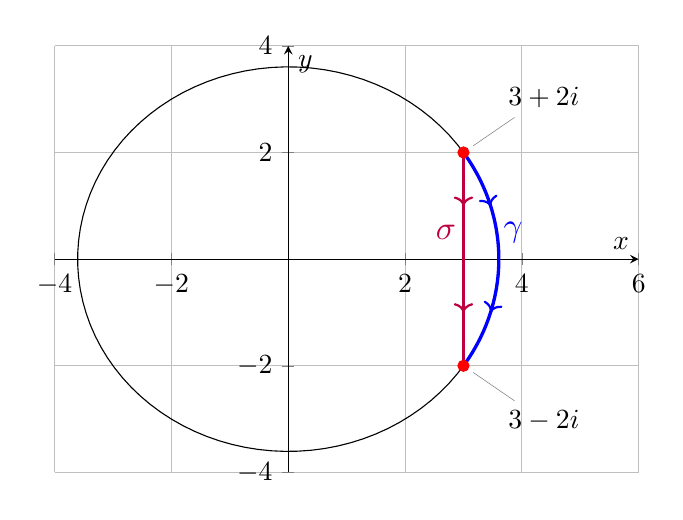
\begin{tikzpicture}
    \begin{axis}[
        axis lines = middle,
        xmin = -4, xmax = 6,
        ymin = -4, ymax = 4,
        xlabel = \(x\),
        ylabel = \(y\),
        width = 9cm,
        height = 7cm,
        grid = both,
    ]
    
    % Draw the full circle
    \addplot [
        domain=0:360,
        samples=100,
        no markers
    ]
    (
        {sqrt(13)*cos(x)},
        {sqrt(13)*sin(x)}
    );
    
    % Highlight the portion between (3, 2i) and (3, -2i)
    \addplot [
        domain=-33.7:33.7,  % Arc between the two points
        samples=100,
        very thick,
        blue
    ]
    (
        {sqrt(13)*cos(x)},
        {sqrt(13)*sin(x)}
    );
    % Add markers and labels for the points (3, 2i) and (3, -2i)
    \addplot [
        only marks,
        mark=*, 
        color=red
    ]
    coordinates {(3, 2) (3, -2)};
    \node at (axis cs:3,2) [pin=above right:{\(3 + 2i\)}] {};
    \node at (axis cs:3,-2) [pin=below right:{\(3 - 2i\)}] {};

    % Add the purple line segment between the two points
    \addplot [
        thick,
        color=purple
    ]
    coordinates {(3, 2) (3, -2)};

    % Add the label for sigma without a marker
    \node at (axis cs:2.7, 0.5) [text=purple, scale=1.2] {\(\sigma\)};
    \node at (axis cs:3.85, 0.5) [text=blue, scale=1.2] {\(\gamma\)};

    \addplot[domain=32:16, thick, blue, ->] 
    ({sqrt(13)*cos(x)}, {sqrt(13)*sin(x)});

    \addplot[domain=0:-16, thick, blue, ->] 
        ({sqrt(13)*cos(x)}, {sqrt(13)*sin(x)});

    \draw[thick, purple, ->] (3,2) -- (3,1);
    \draw[thick, purple, ->] (3,0) -- (3,-1);

    \end{axis}
\end{tikzpicture}

Let us define \(\sigma := \overline{\left[3+2i,3-2i\right]}\) which notice has the same orientation and endpoints as \(\gamma\).

We can parameterise the line segment \(\sigma\) as:

\[
\sigma(t) := 3+2i + t\left(3-2i - \left(3+2i\right)\right) \quad \left(t\in\left[0,1\right]\right)\]
\[
= 3+2i - t\left(4i\right) \quad \left(t\in\left[0,1\right]\right)
\]

Now from \(\textbf{Corollary 8.2}\) we obtain:

\[
\int_{\gamma} f(z)\,dz = \int_{\sigma} f(z) \, dz = \int_{\overline{\left[3+2i,3-2i\right]}} f(z) \, dz = \int_{\overline{\left[3+2i,3-2i\right]}} \left(z-3\right)^8 \, dz  
\]

\[
= \int_{0}^{1} \left(\left(3+2i -4ti\right) -3 \right)^8 \cdot \left(-4i\right) \, dt 
\]
\[
= -4i \int_{0}^{1} \left(2i-4ti\right)^8 \, dt
\]

\[
= -4i \int_{0}^{1} \left(2-4t\right)^8 \, dt
\]
\[
= 4i \left[\frac{\left(2-4t\right)^9}{9}\right]_{0}^{1}
\]
\[
= 4i \left[\frac{\left(-2\right)^9}{9} - \frac{2^9}{9}\right]
\]
\[
= - \frac{1024}{9}i
\] 

Alternatively we can again apply the FTC (\(\textbf{Theorem 8.3}\)), by noticing that \(f = \left(z-3\right)^8\) is continuous on \(\mathbb{C} \supset \gamma\) by the continuity of polynomials. There also exists \(F\) such that  \(F' = f\) and therefore, \(\int_{\gamma} \left(z-3\right)^8 \, dz = F(3+2i) - F(3-2i) = \left[\frac{\left(z-3\right)^9}{9}\right]_{0}^{1} = -\frac{1024}{9}i \) as we found above.

\item We begin by noticing that \(f\) is continuous on \(\mathbb{C} \supset \gamma\) as it is composed of a composition of continuous functions. Our first aim is to find \(F\) such that \(F' = f\) as we can then we can apply the FTC (\(\textbf{Theorem 8.3}\)) which tells us \(\int_{\gamma} f(z) \, dz = F(\gamma(b)) - F(\gamma(a))\).\newline
    \linebreak
    We begin by making the u-substitution \(u = \sin(s) \implies du = \cos(s)ds\)
    \[ \implies \int_{a}^{z} \cos(s) e^{i\pi \sin(s)} \, ds = \int_{sin(a)}^{sin(z)} e^{i\pi u} \,du = \left[\frac{-i}{\pi}e^{i\pi u}\right]_{sin(a)}^{sin(z)}  \]
    \[= \frac{-i}{\pi}e^{i\pi \sin(z)} +  \frac{i}{\pi}e^{i\pi \sin(a)} = \frac{-i}{\pi}e^{i\pi \sin(z)} + a_0 = F(z) \quad \left(\text{where }\frac{i}{\pi}e^{i\pi \sin(a)} = a_0 \in \mathbb{C}\right)\]
    Notice that this \(F\) satisfies the condition \(F' = f\)\newline
    \linebreak
    We have \(\gamma(0) = 0 \) and \(\gamma(1) = \frac{\pi}{2}\)
    \[\implies \int_{\gamma} \cos(z) e^{i\pi \sin(z)} \, dz = F(\gamma(1)) - F(\gamma(0)) = F(\frac{\pi}{2}) - F(0)\]
    Now applying Euler's identity, we get:
    \[  F(\frac{\pi}{2}) - F(0) = \frac{-1}{\pi}\cdot-1 + \frac{i}{\pi}\cdot1 = \frac{i}{\pi} + \frac{i}{\pi} = \frac{2i}{\pi}\] 

\end{enumerate}
\[\]
\textbf{Q3.} Evaluate the following integrals:
\begin{itemize}
    \item[(i)] \(\int_{\gamma} \frac{e^z}{z^3 + 1} \, dz\) where \(\gamma\) is a curve going once anti-clockwise around a triangle with vertices \(1\), \(2 - i\), and \(3 + 2i\).
    \item[(ii)] \(\int_{\gamma} \frac{1}{\cos(z)} \, dz\) where \(\gamma\) is a curve going once anti-clockwise around the boundary of the coordinate rectangle \(R\) having opposite corners \(-1 - 3i\) and \(1 + 3i\).
\end{itemize}

\noindent \textit{Note: The intention is that you only use lecture content up to and including section 8 for this question.}

\noindent \begin{enumerate}[label=\textbf{(\roman*)}]
\item Notice \(z^3 + 1 = 0 \iff z = -1, \frac{1-\sqrt{3}}{2} i, \frac{1+\sqrt{3}}{2} i \)\newline
\linebreak
So \(f\) is holomorphic in \(\mathbb{C} \setminus \{-1,\frac{1-\sqrt{3}}{2} i, \frac{1+\sqrt{3}}{2} i\}\) or more specifically we can say that \(f\) is holomorphic in the open disk, \(D(10+0i,9.2)\). 

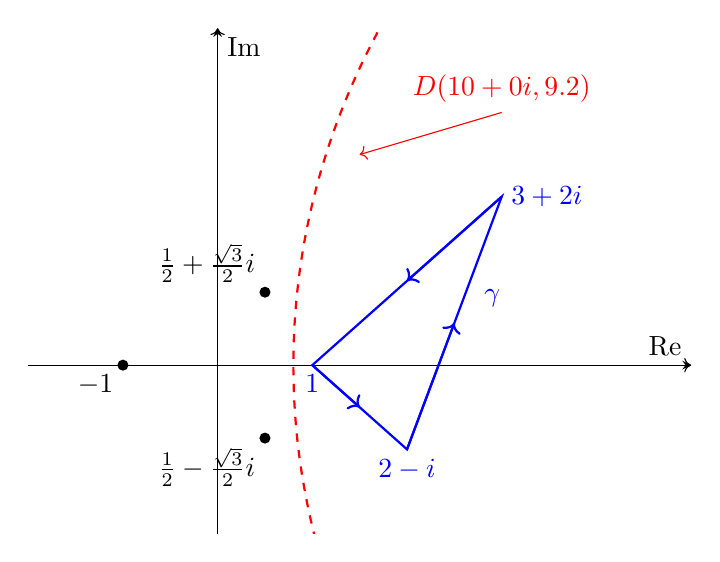
\begin{tikzpicture}
    \begin{axis}[
        width = 10cm,
        height = 8cm,
        axis lines=middle,
        xlabel={Re},
        ylabel={Im},
        xmin=-2, xmax=5,
        ymin=-2, ymax=4,
        xtick=\empty,
        ytick=\empty
        ]
    \clip (-2,-2) rectangle (5,4);

    % Draw the complex plane axes
    \draw[->] (-2, 0) -- (5, 0); % Real axis
    \draw[->] (0, -2) -- (0, 4); % Imaginary axis
    
    % Define the vertices of the triangle
    \coordinate (A) at (1, 0);        % Vertex 1
    \coordinate (B) at (2, -1);       % Vertex 2 - i
    \coordinate (C) at (3, 2);        % Vertex 3 + 2i
    
    % Define the additional points
    \coordinate (D) at (-1, 0);                   % (-1, 0)
    \coordinate (E) at (0.5, -1.732/2);           % 1/2 - sqrt(3)/2 * i
    \coordinate (F) at (0.5, 1.732/2);            % 1/2 + sqrt(3)/2 * i
    
    % Draw the triangle
    \draw[thick, blue] (A) -- (B) -- (C) -- cycle;
    
    % Draw arrows to indicate anti-clockwise direction
    \draw[->, thick, blue] (A) -- ($(A)!0.5!(B)$); % arrow from A to B
    \draw[->, thick, blue] (B) -- ($(B)!0.5!(C)$); % arrow from B to C
    \draw[->, thick, blue] (C) -- ($(C)!0.5!(A)$); % arrow from C to A

    % Label the vertices of the triangle
    \node[below, blue] at (A) {1};
    \node[below,blue] at (B) {$2 - i$};
    \node[right,blue] at (C) {$3 + 2i$};
    
    % Draw and label the additional points
    \fill (D) circle (2pt);
    \node[below left] at (D) {$-1$};

    \fill (E) circle (2pt);
    \node[below left] at (E) {$\frac{1}{2} - \frac{\sqrt{3}}{2}i$};

    \fill (F) circle (2pt);
    \node[above left] at (F) {$\frac{1}{2} + \frac{\sqrt{3}}{2}i$};

    % Draw a circle with center at (10,0) and radius 9
    \draw[thick,dashed, red] (10,0) circle (9.2);

    % Label the center of the circle
    \node[right] at (10,0) {$(10, 0)$};

    \node[above, red] at (3, 3) {$D(10+0i, 9.2)$};

    \draw[->, red] (3,3) -- (1.5,2.5);  
    \node[blue, very thick] at (2.9,0.8) {\(\gamma\)};

    \end{axis}
\end{tikzpicture}

\noindent Now we can apply Cauchy's theorem (\(\textbf{Theorem 8.1}\)) and state that as \(f\) is holomorphic in \(D\) and \(\gamma \) is closed in D, we have:
\[\int_{\gamma} \frac{e^z}{z^3 + 1} \, dz = 0\]
\item We have \(\cos(z) = 0 \iff z = \frac{\pi}{2} + n\pi \quad \forall n \in \mathbb{Z}\)\newline
\linebreak
So \(f\) is holomorphic in \(\mathbb{C} \setminus \{\frac{\pi}{2} + n\pi \quad \forall n \in \mathbb{Z}\}\) or more specifically we can say that \(f\) is holomorphic in the open set U := \(\text{Rec}\left(-1.5-4i, 1.5, 4i\right)\) as \(U \cap \left(\mathbb{C} \setminus \{\frac{\pi}{2} + n\pi \, \forall n \in \mathbb{Z}\}\right) = \emptyset\). \newline
\linebreak
Note that the choice of U is made arbitrarily to satisfy an open set containing R with \(\left|Re(z)\right| < \frac{\pi}{2} \, \forall z \in U.\)

We also notice that the coordinate rectangle \(R := \text{Rec}(-1-3i,1+3i)\) is included in \(U\). I.e \(R \subset U\).\newline
\linebreak
Let us observe the plot of \(R\) and \(U\) on \(\mathbb{C}\):\newline
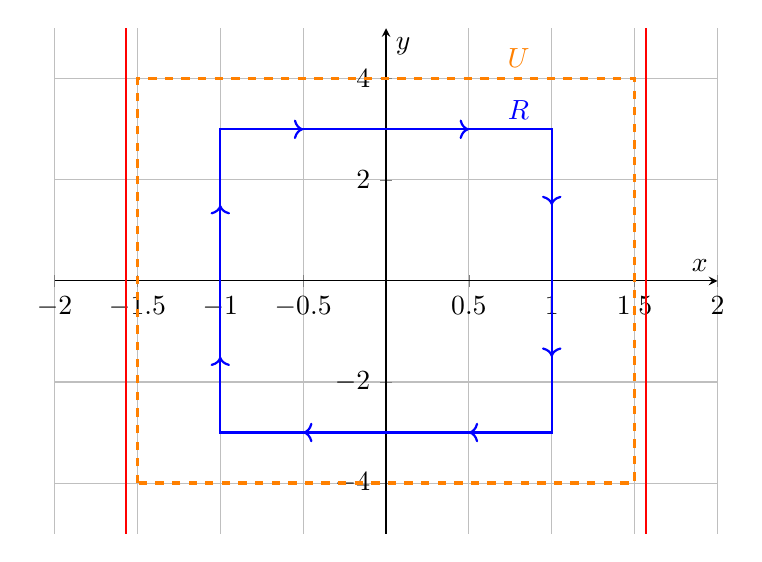
\begin{tikzpicture}
    \begin{axis}[
        axis lines = middle,
        xmin = -2, xmax = 2,
        ymin = -5, ymax = 5,
        xlabel = \(x\),
        ylabel = \(y\),
        width = 10cm,
        height = 8cm,
        grid = both,
    ]
    
    % Draw the rectangle with opposite corners at (-1 - 3i) and (1 + 3i)
    \draw[thick, blue] 
        (axis cs:-1, -3) rectangle (axis cs:1, 3);

     % Add dashed vertical lines at x = pi/2 and x = -pi/2
     \draw[thick, red] 
         (axis cs:-1.57, -5) -- (axis cs:-1.57, 5);
    \draw[thick, red] 
         (axis cs:1.57, -5) -- (axis cs:1.57, 5);    
    
    \node[above, blue] at (0.8, 3) {$R$};

    \draw[thick, blue, ->] (1,3) -- (1,1.5);
    \draw[thick, blue, ->] (1,0) -- (1,-1.5);
    \draw[thick, blue, ->] (1,-3) -- (0.5,-3);
    \draw[thick, blue, ->] (0,-3) -- (-0.5,-3);
    \draw[thick, blue, ->] (-1,-3) -- (-1,-1.5);
    \draw[thick, blue, ->] (-1,0) -- (-1,1.5);
    \draw[thick, blue, ->] (-1,3) -- (-0.5,3);
    \draw[thick, blue, ->] (0,3) -- (0.5,3);


    \draw[dashed,very thick, orange] 
        (axis cs:-1.5, -4) rectangle (axis cs:1.5, 4);
    \node[above,very thick, orange] at (0.8, 4) {$U$};




    \end{axis}
\end{tikzpicture}

We can now apply Goursatt's Lemma (\(\textbf{Lemma 8.10}\)) which tells us that if we have a coordinate rectangle \(R\) in  \(\mathbb{C}\) and \(f\) is holomorphic in an open set \(U \supset R\) then: 
\[
\int_{\partial R} f(z) \, dz = 0
\]

We have shown that \(f\) is holomorphic in the open set \(U \supset R\) and therefore we can conclude by Goursatt's Lemma (\(\textbf{Lemma 8.10}\)) that:

\[
\int_{\partial R} \frac{1}{\cos(z)} \, dz = 0
\]

\end{enumerate}
\[\]
\textbf{Q4.} Let \(p(z)\) be a quadratic polynomial with real coefficients and no real roots. Let \(\gamma\) be a closed curve that goes around both roots in an anti-clockwise direction the same number of times. Prove that

\[
\int_{\gamma} \frac{dz}{p(z)} = 0.
\]
\[\]
\noindent We know that \(p(z)\) has two non-real roots, let us denote these as \(z_1 \text{ and } z_2\).\newline
\linebreak
From this we can express \(p(z)\) as:
\[
p(z) := a\left(z-z_1\right)\left(z-z_2\right) \quad (a \in \mathbb{R})
\]
We now seek to evaluate:
\[
\int_{\gamma} \frac{dz}{p(z)} = \frac{1}{a} \cdot \int_{\gamma} \frac{dz}{\left(z-z_1\right)\left(z-z_2\right)}
\]
\[
=\frac{1}{a} \cdot \int_{\gamma} \left[\frac{a_1}{\left(z-z_1\right)} + \frac{a_2}{\left(z-z_2\right)}\right] \, dz \quad (a_1, a_2 \in \mathbb{C})
\]
\[\]
\noindent We use a partial fraction decomposition to find \(a_1, a_2\):
\[
    \frac{1}{\left(z-z_1\right)\left(z-z_2\right)} = \frac{a_1}{\left(z-z_1\right)} + \frac{a_2}{\left(z-z_2\right)}
\]
\[
\implies 1 = a_1\left(z-z_2\right) + a_2\left(z-z_1\right)
\]
\[
\implies 1 = z\left(a_1 + a_2\right) - \left(a_1z_2 + a_2z_1\right)
\]


\[ \implies
\left\{
\begin{array}{ll}
a_1 + a_2 = 0 \\
a_1z_2 + a_2z_1 = -1
\end{array}
\right.
\]
\[\]
\noindent From this we see \(a_1 = -a_2\) and therefore:

\[
a_2\left(z_1-z_2\right) = -1
\]
\[
\implies a_2 = \frac{1}{z_2-z_1}
\]
\[
\implies a_1 = \frac{1}{z_1-z_2}
\]

\noindent Substituting these coefficients into our expression for \(\frac{1}{p(z)}\) we get:

\[
    \frac{1}{p(z)}=  \frac{1}{a} \cdot \left[\frac{\frac{1}{z_1-z_2}}{z-z_1} + \frac{\frac{1}{z_2-z_1}}{z-z_2} \right]
\]

\[
= \frac{1}{a} \cdot \frac{1}{z_1-z_2} \cdot \left[\frac{1}{z-z_1} - \frac{1}{z-z_2}\right]
\]

\noindent We now reconsider our integral:

\[
    \int_{\gamma} \frac{dz}{p(z)} =\frac{1}{a} \cdot \frac{1}{z_1-z_2} \cdot \int_{\gamma} \left[\frac{1}{z-z_1} - \frac{1}{z-z_2}\right] \, dz
\]

\[
= \frac{1}{a} \cdot \frac{1}{z_1-z_2} \cdot \left[\int_{\gamma} \frac{dz}{z-z_1} \,  - \int_{\gamma} \frac{dz}{z-z_2} \,  \right]
\]

\[
= \frac{1}{a} \cdot \frac{1}{z_1-z_2} \cdot \left[2\pi i \cdot \mathbf{n}\left(\gamma ;z_1\right)  - 2\pi i \cdot \mathbf{n}\left(\gamma ;z_2\right)\right]
\]

\noindent As per \(\textbf{Q4}\), we know that the curve \(\gamma\) goes around \(z_1\) and \(z_2\) in an anti-clockwise direction the same number of times. Let us denote this winding number with \(k\).\newline
\linebreak
\noindent We now have: 
\[
    \int_{\gamma} \frac{dz}{p(z)} = \frac{1}{a} \cdot \frac{1}{z_1-z_2} \cdot \left[2\pi i \cdot k - 2\pi i \cdot k\right]
\]

\[
    = \frac{1}{a} \cdot \frac{1}{z_1-z_2} \cdot 0 = 0 \quad \text{ as required.} \quad \Box
\]
\[\]
\textbf{Q5.} Use winding numbers to evaluate the following integrals:
\begin{itemize}
    \item[(i)] \(\int_{\gamma} \frac{dz}{z^2 - 1}\) where \(\gamma(t) = 1 + t(1 - t) + e^{4\pi it}\) for \(t \in [0, 1]\).
    \item[(ii)] \(\int_{\gamma} \frac{dz}{z^3 - z^2 + 4z - 4}\) where \(\gamma\) goes once anti-clockwise around the circle of radius 3 centred at \(2 + i\).
\end{itemize}

\noindent \begin{enumerate}[label=\textbf{(\roman*)}]
\item We begin by considering the partial fraction decomposition of \(\frac{1}{z^2-1}\)
\[
\frac{1}{z^2-1} = \frac{1}{\left(z-1\right)\left(z+1\right)} = \frac{a}{z-1} + \frac{b}{z+1}
\]

\[
\implies 1 = a\left(z+1\right) + b\left(z-1\right)
\]
\[
\implies 1 = z\left(a+b\right) + \left(a-b\right)
\]
\[ \implies
\left\{
\begin{array}{ll}
a + b = 0 \\
a - b = 1
\end{array}
\right.
\]
\[
\implies a = \frac{1}{2},\quad b=\frac{-1}{2}
\]

\noindent So we now have:

\[
    \int_{\gamma} \frac{dz}{z^2 - 1} = \int_{\gamma} \left[ \frac{1}{2\left(z-1\right)}  - \frac{1}{2\left(z+1\right)} \right] \, dz
\]

\[
= \frac{1}{2} \int_{\gamma} \frac{dz}{z-1} - \frac{1}{2} \int_{\gamma} \frac{dz}{z+1}
\]

\[
= \frac{1}{2} \cdot 2\pi i \cdot \mathbf{n}\left(\gamma;1\right) - \frac{1}{2} \cdot 2\pi i \cdot \mathbf{n}\left(\gamma;-1\right)
\]

\[
  =\pi i \cdot \mathbf{n}\left(\gamma;1\right) -\pi i \cdot \mathbf{n}\left(\gamma;-1\right)
\]

\noindent Let us now compute these two winding numbers:

\[
\mathbf{n}\left(\gamma;1\right) = \frac{1}{2\pi i} \int_{\gamma} \frac{1}{z-1} \, dz
\]

\[
    = \frac{1}{2\pi i} \int_{0}^{1} \frac{1}{\left(1+t\left(t-1\right)+e^{4\pi i t}\right)-1} \cdot \left(1-2t + 4\pi it e^{4\pi it}\right)\, dt
\]

\[
    = \frac{1}{2\pi i} \int_{0}^{1} \frac{1-2t + 4\pi it e^{4\pi i}}{t\left(t-1\right)+e^{4\pi i t}} \, dt
\]

\[
    = \frac{1}{2\pi i} \left[ \ln\left( t\left(t-1\right)+e^{4\pi i t}\right) \right]_{0}^{1}
\]

\[
= \frac{1}{2\pi i} \left[4\pi i - \ln\left(1\right)  \right] = \frac{4\pi i}{2\pi i} = 2
\]

\[
    \mathbf{n}\left(\gamma;-1\right) = \frac{1}{2\pi i} \int_{\gamma} \frac{1}{z+1} \, dz
\]


\[
    = \frac{1}{2\pi i} \int_{0}^{1} \frac{1}{\left(1+t\left(t-1\right)+e^{4\pi i t}\right)+1} \cdot \left(1-2t + 4\pi it e^{4\pi it}\right)\, dt
\]

\[
    = \frac{1}{2\pi i} \int_{0}^{1} \frac{1-2t + 4\pi it e^{4\pi it}}{2+t\left(t-1\right)+e^{4\pi i t}} \, dt
\]

\[
    = \frac{1}{2\pi i} \left[ \ln\left(2+ t\left(t-1\right)+e^{4\pi i t}\right) \right]_{0}^{1}
\]

\[
= \frac{1}{2\pi i} \left[\ln\left(2+e^{4\pi i}\right) - \ln\left(3\right)  \right]= \frac{1}{2\pi i} \left[\ln\left(3\right) - \ln\left(3\right)  \right] = 0
\]

\noindent So we now have: 

\[
    \int_{\gamma} \frac{dz}{z^2 - 1}  =\pi i \cdot \mathbf{n}\left(\gamma;1\right) -\pi i \cdot \mathbf{n}\left(\gamma;-1\right) = \left[2\right]\pi i - \left[0\right]\pi i = 2\pi i
\]
\[\]
\noindent Let us observe these winding numbers on the plot of:
 \[\gamma(t) = 1 + t(1 - t) + e^{4\pi it} \text{ for } t \in [0, 1] \]

%\begin{tikzpicture}
    %\begin{axis}[
     %   trig format plots=rad,
      %  axis equal,
      % hide axis
   % ]
    
   % \addplot [domain=0:1,samples=200, red]({1 + t*(1 - t) + cos(4*3.1415* t)},{sin(4*3.1415*t)});
   % \end{axis}
  %  \end{tikzpicture}

  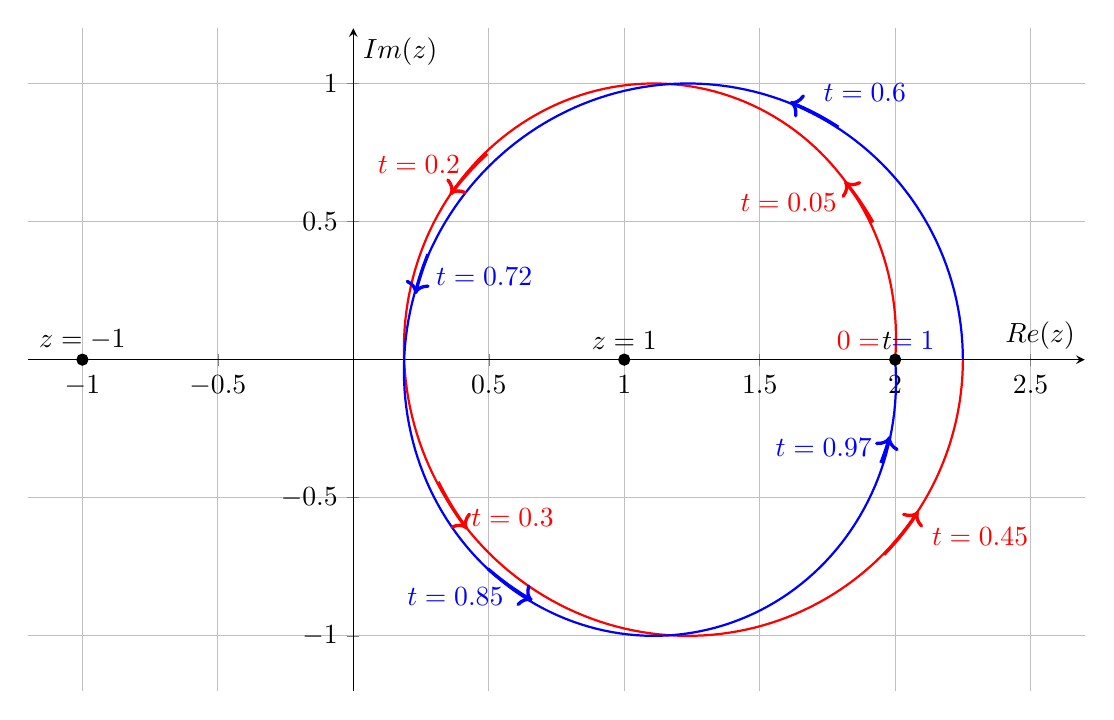
\begin{tikzpicture}
    \begin{axis}[
        axis lines=middle,
        trig format plots = rad,
        xlabel={$Re(z)$},
        ylabel={$Im(z)$},
        domain=0:1,
        xmin = -1.2, xmax = 2.7,
       % xmin = -6, xmax = 6,
        ymin = -1.2, ymax = 1.2,
       % ymin = -5, ymax = 5,
        samples=200,
        width=15cm,
        height=10cm,
        legend pos=outer north east,
        grid=both
    ]
        \addplot [
            domain=0:0.5,
            samples=200,
            red,
            thick
        ]
        ({1 + x*(1-x) + cos(4*pi*x)}, {sin(4*pi*x)});
        \addplot [
            domain=0.5:1,
            samples=200,
            blue,
            thick
        ]
        ({1 + x*(1-x) + cos(4*pi*x)}, {sin(4*pi*x)});
    
    \addplot[domain=0.52:0.7, very thick, red, ->] 
    ({1.05+cos(x)}, {sin(x)});

    \addplot[domain=2.3:2.5, very thick, red, ->] 
        ({1.16+cos(x)}, {sin(x)});
    \addplot[domain=4:4.2, very thick, blue, ->] 
        ({1.15+cos(x)}, {sin(x)});
    \addplot[domain=5.5:5.7, very thick, red, ->] 
        ({1.25+cos(x)}, {sin(x)});
    
   
    \addplot[domain=3.6:3.8, very thick, red, ->] 
        ({1.21+cos(x)}, {sin(x)});
    \addplot[domain=5.90:6, very thick, blue, ->] 
        ({1.02+cos(x)}, {sin(x)});
    \addplot[domain=1:1.2, very thick, blue, ->] 
        ({1.25+cos(x)}, {sin(x)});
    \addplot[domain=2.75:2.9, very thick, blue, ->] 
        ({1.20+cos(x)}, {sin(x)});

    \node[above left, red] at (1.98, 0) {$0 =$};
    \node[above left, red] at (1.82, 0.5) {$t=0.05$};
    \node[above left, red] at (0.43, 0.64) {$t=0.2$};
    \node[above right, red] at (0.4, -0.64) {$t=0.3$};
    \node[right, red] at (2.1, -0.64) {$t=0.45$};
    \node[above right, blue] at (1.7, 0.9) {$t=0.6$};
    \node[right, blue] at (0.27, 0.3) {$t=0.72$};
    \node[below left, blue] at (0.59, -0.79) {$t=0.85$};
    \node[below left, blue] at (1.95, -0.25) {$t=0.97$};
    \node[above right, blue] at (1.95,0) {$= 1$};
    \node[above, black] at (1.97, 0) {$t$};
    \addplot[only marks, mark=*, black] 
    coordinates {(2,0) (-1,0) (1,0)};
    \node[above, black] at (1, 0) {$z=1$};
    \node[above, black] at (-1, 0) {$z=-1$};

    \end{axis}
    \end{tikzpicture}


\noindent Notice \(\gamma\) goes around \(z=1\) twice in an anticlockwise direction but does not go around \(z=-1\).  \newline
\linebreak
Hence \(\mathbf{n}\left(\gamma;1\right) = 2 \text{ and } \mathbf{n}\left(\gamma;-1\right) = 0 \) as previously shown.
\[\]
\item We begin by considering the partial fraction decomposition of \(\frac{1}{z^3 - z^2 + 4z - 4}\)

\[
\frac{1}{z^3-z^2+4z-4} = \frac{1}{\left(z-1\right)\left(z-2i\right)\left(z+2i\right)} = \frac{a}{z-1} + \frac{b}{z-2i} + \frac{c}{z+2i}
\]

\[
\implies 1 = a\left(z-2i\right)\left(z+2i\right) + b\left(z-1\right)\left(z+2i\right) + c\left(z-1\right)\left(z-2i\right)
\]

\[
\implies 1 = z^2\left(a+b+c\right) + z\left(2ib -b -2ic -c\right) + \left(4a-2ib+2ic\right)
\]
\[ \implies
\left\{
\begin{array}{lll}
a+b+c=0 \\
2ib -b-2ic -c = 0 \\
4a - 2ib + 2ic = 1
\end{array}
\right.
\]
\[
\implies \begin{pmatrix}
1 & 1 & 1 \\
0 & 2i - 1 & -2i - 1 \\
4 & -2i & 2i
\end{pmatrix}
\begin{pmatrix}
a \\
b \\
c
\end{pmatrix}
=
\begin{pmatrix}
0 \\
0 \\
1
\end{pmatrix}
\]

\[
\implies 
\begin{pmatrix}
a \\
b \\
c
\end{pmatrix}
=
\begin{pmatrix}
1 & 1 & 1 \\
0 & 2i - 1 & -2i - 1 \\
4 & -2i & 2i
\end{pmatrix}^{-1}
\begin{pmatrix}
0 \\
0 \\
1
\end{pmatrix}
\]

\[
\implies \begin{pmatrix}
    a \\
    b \\
    c
    \end{pmatrix}
    =\frac{1}{20}
    \begin{pmatrix}
    4 & 4 & 4 \\
    8-4i &-2-4i & -2+i \\
    8+4i & -2+4i & -2-i 
    \end{pmatrix}
    \begin{pmatrix}
    0 \\
    0 \\
    1
    \end{pmatrix}
\]



\[
\implies \begin{pmatrix}
    a \\
    b \\
    c
    \end{pmatrix}
    =\frac{1}{20}
    \begin{pmatrix}
    4 \\
    -2+i \\
    -2-i 
    \end{pmatrix}
    =
    \begin{pmatrix}
       \frac{1}{5} \\
        -\frac{1}{10}+\frac{i}{20} \\
        -\frac{1}{10}-\frac{i}{20} 
        \end{pmatrix}
\]

So we now have:

\[
\int_{\gamma} \frac{dz}{z^3 - z^2 + 4z - 4} = \int_{\gamma} \left[\frac{1}{5\left(z-1\right)} - \frac{2+i}{20\left(z+2i\right)} - \frac{2-i}{20\left(z-2i\right)}\right] \, dz
\]

\[
= \frac{1}{5}\int_{\gamma} \frac{dz}{z-1} - \frac{2+i}{20} \int_{\gamma} \frac{dz}{z+2i}\, dz - \frac{2-i}{20} \int_{\gamma} \frac{dz}{z-2i}
\]

\[
= \frac{1}{5}\left(2\pi i\right) \mathbf{n}\left(\gamma;1\right) - \frac{2+i}{20} \left(2\pi i\right) \mathbf{n}\left(\gamma;-2i\right)- \frac{2-i}{20} \left(2\pi i\right)\mathbf{n}\left(\gamma;2i\right)
\]
\noindent We know \(\gamma\) only goes once around the circle \(C(2+i;3)\) and it does so anti-clockwise. Therefore, each winding number will be either \(1\) or \(0\) depending on whether the point is contained within \(C(2+i;3)\).\newline
\linebreak
Firstly consider the point \(z=1\):
\[
    \left| 1 - \left(2+i\right) \right| = \left| - 1 - i \right| = \sqrt{2} < 3.
\]
\[
    \implies \text{The point } z = 1 \text{ is contained within } C(2+i;3)
\]
\[
\text{Hence } \mathbf{n}\left(\gamma;1\right) = 1
\]

Secondly consider the point \(z=-2i\):
\[
    \left| -2i - \left(2+i\right) \right| = \left| - 2 - 3i \right| = \sqrt{13} > 3.
\]
\[
    \implies \text{The point } z = -2i \text{ is not contained within } C(2+i;3)
\]
\[
    \text{Hence } \mathbf{n}\left(\gamma;-2i\right) = 0
\]

Finally consider the point \(z=2i\):
\[
    \left| 2i - \left(2+i\right) \right| = \left| - 2 + i \right| = \sqrt{5} < 3.
\]
\[
    \implies \text{The point } z = 2i \text{ is contained within } C(2+i;3)
\]
\[
    \text{Hence } \mathbf{n}\left(\gamma;2i\right) = 1
\]

Therefore, we can conclude that:
\[
\int_{\gamma} \frac{dz}{z^3 - z^2 + 4z - 4} = \frac{1}{5}\left(2\pi i\right) \mathbf{n}\left(\gamma;1\right) - \frac{2+i}{20} \left(2\pi i\right) \mathbf{n}\left(\gamma;-2i\right)- \frac{2-i}{20} \left(2\pi i\right)\mathbf{n}\left(\gamma;2i\right)
\]

\[
    = \frac{1}{5}\left(2\pi i\right) \mathbf{n}\left(\gamma;1\right) - \frac{2-i}{20} \left(2\pi i\right)\mathbf{n}\left(\gamma;2i\right)
\]

\[
=2\pi i\left[\frac{1}{5} \mathbf{n}\left(\gamma;1\right) - \frac{2-i}{20} \mathbf{n}\left(\gamma;2i\right)\right]
\]

\[
=2\pi i\left[\frac{1}{5} - \frac{2-i}{20}\right]
\]

\[
= 
2\pi i\left[\frac{2+i}{20}\right] 
\]

\[
= 
\pi i\left[\frac{2+i}{10}\right] 
\]

\[
= 
\frac{2\pi i}{10} - \frac{\pi}{10}
\]

\[
= \frac{\pi}{10} \left[2i - 1\right]
\]

\end{enumerate}    
\hrulefill

\end{document}

